\section{Contribution}\label{contribution}

%The previous work on model typing \cite{ecmfa12} introduces substitutability into model types, and formally defines a subtyping relation between two model types specified using MOF\cite{MOF}.
%The previous work, however, only considers MOF-based structural subtyping in which the structure of two model types determines whether one is subtype of the other, which limits the applicability of model subtyping in a setting where OCL contracts are needed to precisely define modeling languages (e.g., specifying a model transformation).

In this paper we extend the subtyping relation described in \cite{ecmfa12} by taking into account OCL contracts for a safe substitutability of models conforming to metamodels including contracts. This provides a safe reuse of model transformations expressed on metamodels that include contracts. 
Specifically, we extend the MOF class matching (cf. Def. 2 of Section \ref{background}) by considering contracts matching (Section \ref{classmatching}) and provide a technique for analyzing the matching of OCL contracts associated with two classes with different model types (Section \ref{analyzingcontract}). In this section we describe the contract matching technique we developed to support contract-aware model substitutability. We also describe an Alloy-based prototype tool that supports contract matching (Section \ref{toolsupport}), and illustrate the use of contract-aware substitutability using the motivating examples (Section \ref{casestudy}).    

\subsection{Contract-aware MOF Class Matching}\label{classmatching}

We consider the use of OCL invariants added to MOF classes to specify additional structural properties, and OCL pre-/post-conditions defined in the context of MOF class operations to specify the model manipulation rules (e.g., transformation) associated with model types. 
The MOF class matching relation is thus determined by two aspects: the structural features specified using MOF (e.g., classes, properties, operation signatures, etc.) and the contracts expressed using OCL (e.g., invariants and pre-/post-conditions).  
%While the previous work \cite{ecmfa12} used the structural elements (cf. Def. 3 of \cite{ecmfa12}) to determine the matching relation between two MOF classes, the focus of this paper is to provide a formal definition of the contract matching used to support the contract-aware MOF class matching.  

The substitutability through model subtyping is a specialization of the Liskov Substitution Principle \cite{liskov1994behavioral} on the model type system. 
Specifically the contract matching relation that enables contract-aware model substitutability must abide by the following rules: (1) invariants of the supermodel type cannot be weakened in a sub model type, (2) pre-conditions cannot be strengthened in a sub model type, and (3) post-conditions cannot be weakened in a sub model type.
The extended MOF class matching relation is formalized as follows:

\begin{definition}[Contract-aware MOF Class Matching] Class $T'$ matches T (written $T'$ <\# T) iff their structures match (cf. Def. 3 of \cite{ecmfa12}), their invariants match and their operation pre-/post-conditions match, where
\begin{enumerate}
\item[1] \textbf{Invariants Match} is defined as follows:\\
let T.ownedInvariant = $\{$$inv_{T1}$, $inv_{T2}$, ..., $inv_{Tk}$ $\}$ be the invariants defined for $T$;\\
let $result_T$ = $inv_{T1}$ $\wedge$ $inv_{T2}$ $\wedge$ ... $\wedge$ $inv_{Tk}$;\\
let SuperClass(T) = $\{$$cls_1$, $cls_2$, ..., $cls_n$$\}$ where $cls_i$ is a superclass of T; \\
let $cls_i$.ownedInvariant = $\{$ $inv_{i1}$, $inv_{i2}$, ..., $inv_{ik}$ $\}$ be the invariants defined for $cls_i$, for i = 1, .., n;\\
let $result_i$ = $inv_{i1}$ $\wedge$ $inv_{i2}$ $\wedge$ ... $\wedge$ $inv_{ik}$, for i = 1, .., n;\\
let invs = $result_1$ $\wedge$ $result_2$ $\wedge$ ... $\wedge$ $result_n$ $\wedge$ $result_T$;\\
\\
let T$'$.ownedInvariant = $\{$$inv'_{T1}$, $inv'_{T2}$, ..., $inv'_{Tk}$ $\}$ be the invariants defined for $T'$;\\
let $result'_T$ = $inv'_{T1}$ $\wedge$ $inv'_{T2}$ $\wedge$ ... $\wedge$ $inv'_{Tk}$;\\
let SuperClass(T$'$) = $\{$$cls'_1$, $cls'_2$, ..., $cls'_n$$\}$ where $cls'_i$ is a superclass of T$'$; \\
let $cls'_i$.ownedInvariant = $\{$ $inv'_{i1}$, $inv'_{i2}$, ... , $inv'_{ik}$ $\}$ be the invariants defined for $cls'_i$, for i = 1, .., n;\\
let $result'_i$ = $inv'_{i1}$ $\wedge$ $inv'_{i2}$ $\wedge$ ... $\wedge$ $inv'_{ik}$, for i = 1, .., n;\\
let invs$'$ = $result'_1$ $\wedge$ $result'_2$ $\wedge$ ... $\wedge$ $result'_n$ $\wedge$ $result'_T$;\\
\\
The invariants of T and T$'$ match if Models(invs) $\supseteq$ Models(invs$'$), where $Models(invs)$ returns all models that satisfy $invs$ and $Models(invs')$ returns all models that satisfy $invs'$.\\
%\begin{algorithmic}
%\State let result1 = true, result2 = true, invs = true, invs$'$ = true
%\For {each cls in SuperClass(T)}
%    \For {each inv in cls.ownedInvariant} 
%		 		\State {result1 = result1 $\wedge$ inv}
%    \EndFor 
%    \State {invs = invs $\wedge$ result1}
%\EndFor 
%\For {each cls$'$ in SuperClass(T$'$)}
%    \For {each inv$'$ in cls$'$.ownedInvariant} 
%		 		\State {result2 = result2 $\wedge$ inv$'$}
%    \EndFor 
%    \State {invs$'$ = invs$'$ $\wedge$ result2}
%\EndFor 

%\State Models(invs) $\supseteq$ Models(invs$'$)
%\end{algorithmic}

%let invs: Constraint = SuperClasses(T)$\rightarrow$iterate(cls: Class, result1 : Constraint = true $|$ result1 and cls.ownedInvariant$\rightarrow$iterate(inv: Constraint, result2 : Constraint = true$|$ result2 and inv)),\\ 
%let invs$'$: Constraint = SuperClasses(T$'$)$\rightarrow$iterate(cls: Class, result1 : Constraint = true$|$ result1 and  cls.ownedInvariant$\rightarrow$iterate(inv: Constraint, result2 : Constraint = true $|$ result2 and inv)),\\
%invs $\supseteq$ invs$'$\\

%{\em Note that {\em SuperClasses(T)} returns $T$ plus all super classes of $T$.
%$invs$ is the conjunction of the invariants defined in the context of $T$ and its super classes, and $invs'$ is the conjunction of the invariants defined in the context of $T'$ and its super classes.
%{\em Models(invs)} returns all models that satisfy $invs$. 
%The clause {\em Models(invs) $\supseteq$ Models(invs$'$)} specifies that the models satisfying $invs$ must include the models satisfying $invs'$ (i.e., $invs$ are weaker than $invs'$).}\\
 
\item[2] \textbf{Pre-/post-conditions Match} is defined as follows:\\
$\forall$ op $\in$ T.ownedOperation, $\exists$ $S'$ $\in$ SuperClasses($T'$) such that $\exists$ $op'$ $\in$ $S'$.ownedOperation and:\\
	\begin{enumerate}
		\item[2.1] 
		let op.ownedPrecondition = $\{$$pre_{1}$, $pre_{2}$, ..., $pre_{k}$ $\}$ be the pre-conditions defined for $op$;\\
		let pres = $pre_{1}$ $\wedge$ $pre_{2}$ $\wedge$ ... $\wedge$ $pre_{k}$;\\
		let op$'$.ownedPrecondition = $\{$$pre'_{1}$, $pre'_{2}$, ..., $pre'_{k}$ $\}$ be the pre-conditions defined for $op'$;\\
		let pres$'$ = $pre'_{1}$ $\wedge$ $pre'_{2}$ $\wedge$ ... $\wedge$ $pre'_{k}$;\\
		\\
		%\begin{algorithmic}
		%	\State let pres = true, pres$'$ = true,
		%	\For {each pre in op.ownedPrecondition}
		%		\State {pres = pres $\wedge$ pre}
		%	\EndFor
		%	\For {each pre$'$ in op$'$.ownedPrecondition}
		%		\State {pres$'$ = pres$'$ $\wedge$ pre$'$}
		%	\EndFor
		%	\State Models(pres$'$) $\supseteq$ Models(pres)
		%\end{algorithmic}
		
		
		%let pres$'$: Constraint = op$'$.ownedPrecondition$\rightarrow$iterate(pre: Constraint, result : Constraint = true $|$ result and pre), \\
		%let pres : Constraint = op.ownedPrecondition$\rightarrow$iterate(pre: Constraint, result : Constraint = true $|$ result and pre), \\
		%pres$'$ $\supseteq$ pres
		\item[2.2] 
		let op.ownedPostcondition = $\{$$post_{1}$, $post_{2}$, ..., $post_{k}$ $\}$ be the post-conditions defined for $op$;\\
		let posts = $post_{1}$ $\wedge$ $post_{2}$ $\wedge$ ... $\wedge$ $post_{k}$;\\
		let op$'$.ownedPostcondition = $\{$$post'_{1}$, $post'_{2}$, ..., $post'_{k}$ $\}$ be the post-conditions defined for $op'$;\\
		let posts$'$ = $post'_{1}$ $\wedge$ $post'_{2}$ $\wedge$ ... $\wedge$ $post'_{k}$;\\
		\\
		The operation specifications of T and T$'$ match if Models(pres$'$) $\supseteq$ Models(pres) and Models(posts) $\supseteq$ Models(posts$'$)
		%\begin{algorithmic}
		%	\State let posts = true, posts$'$ = true,
		%	\For {each post in op.ownedPostcondition}
		%		\State {posts = posts $\wedge$ post}
		%	\EndFor
		%	\For {each post$'$ in op$'$.ownedPostcondition}
		%		\State {posts$'$ = posts$'$ $\wedge$ post$'$}
		%	\EndFor
		%	\State Models(posts) $\supseteq$ Models(posts$'$)
		%\end{algorithmic}
		
		%let posts$'$: Constraint = op$'$.ownedPostcondition$\rightarrow$iterate(post: Constraint, result : Constraint = true $|$ result and post),\\
		%let posts : Constraint = op.ownedPostcondition$\rightarrow$iterate(post: Constraint, result : Constraint = true $|$ result and post), \\
		%posts	$\supseteq$ posts$'$\\
		\end{enumerate} 	

%{\em Note that $pres$ is the conjunction of pre-conditions defined in the context of $op$, and $pres'$ is the conjunction of the pre-conditions defined in the context of $op'$. The models satisfying $pres'$ must include the models satisfying $pres$.
%$posts$ is the conjunction of post-conditions defined in the context of $op$, and $posts'$ is the conjunction of the post-conditions defined in the context of $op'$. The models satisfying $posts$ must include the models satisfying $posts'$.}

\end{enumerate}

\label{definition1}
\end{definition}

%The extended MOF class matching that enables contract-aware model substitutability can thus be used to determine the subtyping relation between two model types that include contracts .  

\subsection{Analyzing the Matching of Contracts}\label{analyzingcontract}

Definition \ref{definition1} can be used to formally reason about the matching relation between two MOF classes with contracts. 
The MOF class matching relation in Definition \ref{definition1} includes the matching of the contracts from classes of two model types. 
Consequently, analyzing such relations requires one to formally analyze the relation between contracts (e.g., to check if the models satisfying one contract includes the models satisfying the other).
To do this, a query function $Models$($MT$, $C$) is used to compute all models that both conform to a model type $MT$ and satisfy an OCL contract $C$ defined in $MT$. %A contract can be an invariant, a pre-condition or a post-condition. 
Thus given contract $C_1$ in a candidate supermodel type $MT_1$ and contract $C_2$ in a candidate sub model type $MT_2$, $C_1$ matches $C_2$ iff (1) $C_1$, $C_2$ are invariants, and $Models$($MT_1$, $C_1$) $\supseteq$ $Models$($MT_2$, $C_2$), (2) $C_1$, $C_2$ are pre-conditions, and $Models$($MT_2$, $C_2$) $\supseteq$ $Models$($MT_1$, $C_1$), and (3) $C_1$, $C_2$ are post-conditions, and $Models$($MT_1$, $C_1$) $\supseteq$ $Models$($MT_2$, $C_2$). 

Checking the contract matching requires a tool to implement the functionality of the query function $Models$($MT$, $C$).
%For example, given a contract defined in a model type, a tool is needed to generate the models that both conform to the model type and satisfy the contract.
We use the Alloy Analyzer \cite{jackson2002alloy} for this purpose. The Alloy Analyzer is used to analyze Alloy specifications. It is supported by a SAT-based model finder.
The Alloy Analyzer can generate models that conform to a model type expressed in Alloy in terms of signatures and fields that specify the model type structure and a predicate that expresses the contracts. 
In this paper we use the Alloy Analyzer at the back-end to check whether two contracts match.

For example, given a candidate supermodel type $MT_1$ and a candidate sub model type $MT_2$, with two OCL invariants respectively, $C_1$ and $C_2$, the procedure below can be used to check if $C_1$ matches $C_2$.

\begin{enumerate}
\item (preprocess) Since model subtyping requires each element in the supermodel type to be matched by an element in the sub model type (see Definition \ref{definition1}), the contract defined in the supermodel type refers to elements that also exist in the sub model type. 
Thus we can move $C_1$ to $MT_2$, and use only the sub model type (i.e., $MT_2$) to check whether $C_1$ and $C_2$ match.
%move $C_1$ to $MT_2$, and check the relation between $C_1$ and $C_2$ in $MT_2$.
%Note that the procedure described in the paper uses only one model type to check the relation between $C_1$ and $C_2$.
%Note that it is difficult to check the relation between a contract in a super model type and a contract in a submodel type, since the contract in a submodel type may reference structural elements (e.g., MOF classes) that are not included by the super model type.

\item Transform $MT_2$ to an Alloy model using the technique described in \cite{sun2011rigorous}. 
Convert $C_1$ and $C_2$ into two Alloy predicates, $P_1$ and $P_2$, respectively.  

\item Run an empty predicate in the Alloy Analyzer to search for a model conforming to the model type $MT_2$. 
If the Analyzer returns no model satisfying the empty predicate (i.e., $Models$($MT_2$, $\emptyset$) = $\emptyset$), $Models$($MT_2$, $C_1$) = $\emptyset$ and $Models$($MT_2$, $C_2$) = $\emptyset$. In this case $C_1$ matches $C_2$ since $\emptyset$ is a subset of $\emptyset$; otherwise, continue to the next step.  

\item Run $P_1$ and $P_2$ respectively. 
If the Alloy Analyzer returns no model for each predicate (i.e., $Models$($MT_2$, $C_1$) = $\emptyset$ and $Models$($MT_2$, $C_2$) = $\emptyset$), then $C_1$ matches $C_2$; if the Alloy Analyzer returns a model (or models) for only $P_1$, then $C_1$ matches $C_2$; if the Alloy Analyzer returns a model (or models) for only $P_2$, then $C_1$ does not match $C_2$; otherwise, continue to the next step.

\item Run a predicate to search for a model satisfying both $P_1$ and $P_2$. 
If the Alloy Analyzer returns a model satisfying the predicate, continue to the next step; otherwise, $C_1$ does not match $C_2$.

\item Run a predicate $P_3$ to search for a model satisfying both $P_1$ and $\neg{P_2}$ (i.e., the negation of $P_2$), and another predicate $P_4$ to search for a model satisfying both $P_2$ and $\neg{P_1}$. 
If the Alloy Analyzer returns no model for both $P_3$ and $P_4$ (i.e., $Models$($MT_2$, $C_1$) = $Models$($MT_2$, $C_2$)), $C_1$ matches $C_2$; if the Alloy Analyzer returns a model (or models) satisfying only $P_3$, $Models$($MT_2$, $C_1$) $\supset$ $Models$($MT_2$, $C_2$) and $C_1$ matches $C_2$; 
%if the Alloy Analyzer returns a model (or models) satisfying only $P_4$, $Models$($MT_2$, $C_1$) $\subset$ $Models$($MT_2$, $C_2$) and $C_1$ does not match $C_2$; 
otherwise, $C_1$ does not match $C_2$.
\end{enumerate}

%Note that Step 4, 5, and 6 of the above procedure can be skipped if we only check whether $C_1$ includes $C_2$.
%The Alloy keyword ``implies'' (i.e., use $P_2$ $implies$ $P_1$ to check if $C_2$ is included by $C_1$) can be directly used to infer whether $C_1$ includes $C_2$.
The approach uses the Alloy Analyzer at the back-end to analyze the relation between two contracts, and it thus requires a translation from OCL expressions to Alloy specifications.
The OCL to Alloy translation used in the prototype tool we developed is based on translation rules described in work by Bordbar et al. \cite{anastasakis2010challenges}. 

\subsection{Contract Matching Checking Tool}\label{toolsupport}

\begin{figure}[!t]
%\centering
\hspace{-5ex}
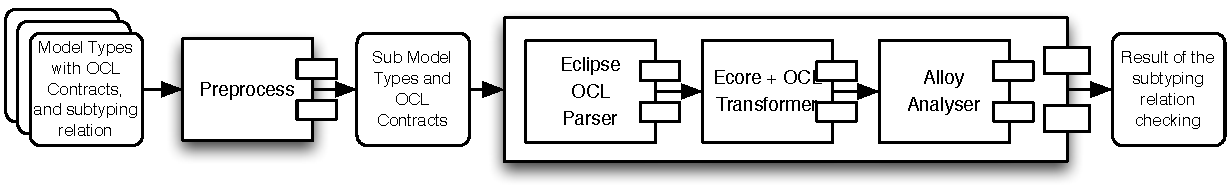
\includegraphics[width=5.3in]{fig/ToolSupport.pdf}
\caption{Contract Matching Checking Tool Overview}
\label{fig:toolsupport}
\end{figure}

The contract matching approach described in the previous subsection has been implemented in a prototype tool.
Figure \ref{fig:toolsupport} shows an overview of the prototype tool.
It consists of an OCL parser, an Ecore\footnote{Ecore is an implementation aligned with MOF included in the Eclipse Modeling Framework \cite{steinberg2008emf}.}/OCL transformer and the use of the Alloy Analyzer.
The Ecore/OCL transformer is developed using Kermeta \cite{muller2005weaving}, an aspect-oriented metamodeling tool. 
The inputs of the prototype are (1) an Ecore file that specifies two model types, and (2) a textual OCL file that specifies the contracts from each model type. 
The model types and contracts are automatically transformed to an Alloy model consisting of signatures and predicates.

The prototype provides several interfaces to check contract matching.
For example, {\em matchInv(inv1: Constraint, inv2: Constraint)} is used to check whether $inv1$ matches $inv2$.
In addition, {\em matchInvs(cls1: Class, cls2: Class)} can be used to check whether the invariants defined in $cls1$ and the invariants defined in $cls2$ match. 
%A relation query is transformed to an Alloy assertion that is added to the generated Alloy model.   

%The prototype then uses the APIs provided by the Alloy Analyzer to pass the Alloy model to the Alloy SAT solver.
%The result returned by the Alloy SAT solver is interpreted by the prototype to get feedback on the relation between two contracts. This relation is then used to check a declared subtyping relation between two model types. 

\subsection{Case Study}\label{casestudy}

In this section we illustrate how to use our approach to define model types and subtyping relations between them to ensure a safe reuse of model transformations.

\subsubsection{A Simple Case Study of Structural Substitutability}

\begin{figure}[!t]
\centering
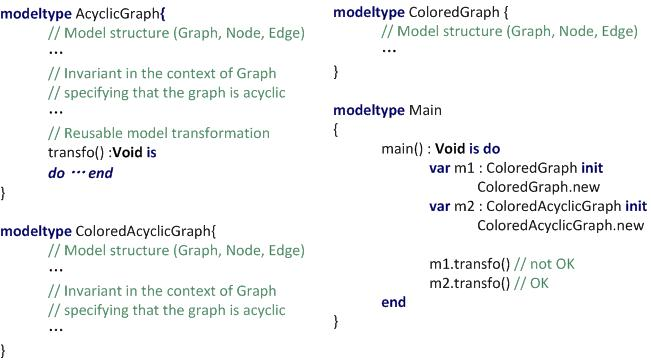
\includegraphics[width=4.8in]{fig/CaseStudy1.jpg}
\caption{A Simple Example of Structural Substitutability in Kermeta}
\label{fig:casestudy1}
\end{figure}

Let us reconsider the scheduling example described in Section \ref{structuralexample}.
A model transformation performs a static scheduling on an acyclic dependence graph.
The model transformation needs a metamodel for ``Acyclic Graph'' (due to space limitation, the metamodel is not shown in the paper).  
The model type $AcyclicGraph$ (see Figure \ref{fig:casestudy1}) shows a simple example of model type definition for the dependency graph used in the example. 
Its definition consists of metaclasses that specify a graph structure, an invariant that specifies the acyclicity property, and a model transformation that takes as input an acyclic graph.

Suppose that in another context a colored graph is used as an intermediate representation and it extends the concept of nodes by introducing additional information. 
To reuse the transformation defined in $AcyclicGraph$, a colored graph must be a subtype of $AcyclicGraph$. 
The model type $ColoredAcyclicGraph$ ensues the subtyping relation by adding an acyclicity invariant in its definition. However, the model type $ColoredGraph$ does not specify any invariants. 
A compilation error will thus show that the $transfo$ operation cannot take as input an instance of $ColoredGraph$ because $ColoredGraph$ is not a subtype of $AcyclicGraph$. 


\subsubsection{A Simple Case Study of Behavioral Substitutability}

\begin{figure}[!t]
\centering
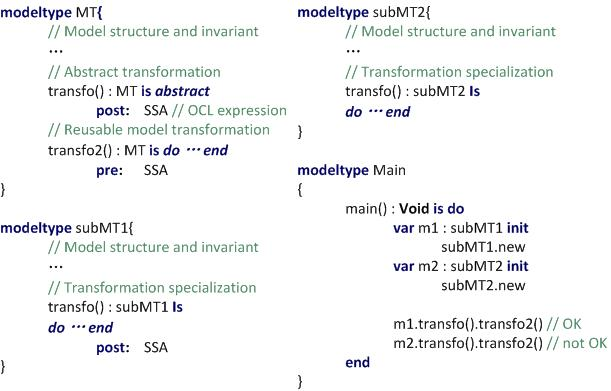
\includegraphics[width=4.8in]{fig/CaseStudy2.jpg}
\caption{A Simple Example of Behavioral Substitutability in Kermeta}
\label{fig:casestudy2}
\end{figure}

In the optimizing compiler community, the daily task for software engineers is to design compilation chains in the right partial order, that is, scheduling the various passes (i.e., optimization, translation, code generation, analysis, etc.).
Designing compilation chains would benefit from behavioral substitutability by opening the way to describe ``abstract'' compilation chains, capitalizing a given knowledge in terms of constraints (pre-/post-conditions) to schedule a set of passes for a given purpose, where each pass would be then implemented in various ways, but conforming to the pre-/post-conditions defined in the abstract compilation chain.    

Figure \ref{fig:casestudy2} shows a simple example of model types used for the compilation chain. 
Suppose that the abstract model transformation $\mathit{transfo}$ defined in $MT$ is used for optimization purpose and define a post condition stating that the model must conform to the Static Single Assignment (SSA) form. $MT$ also contains $\mathit{transfo2}$ as the next pass of the compilation chain and states as precondition that the model must conform to the SSA form. 
The two model types $subMT1$ and $subMT2$ implement the model transformation $\mathit{transfo}$ but only $subMT1$ ensures as postcondition the SSA form. While $subMT2$ is not in this case a sub model type to $MT$, a compilation error for $m2.$$\mathit{transfo}().$$\mathit{transfo}2()$ will be returned. This shows that the model returned by $\mathit{transfo}$ in $subMT2$ (typed by $subMT2$) is not of type $MT$, and can not reuse $\mathit{transfo2}$.